% !TEX root = ../Thesis.tex
\chapter{The Standard Model of Particle Physics} \label{sec:the_standard_model_of_particle_physics}
Particle physics, or high-energy physics, is the study of the most fundamental consituents of matter and their interactions. The best current description of these interactions is known as The Standard Model of Particle Physics (SM); a group of theories that cover all currently known particles and their interactions. The SM was developed through-out the latter half of the 20th century and has seen tremendous success in predicting the behaviour of our universe at the most fundamental level. The SM has stood the test of time and rigorous examination by numerous experiments. Additionally many of its parameters have been measured with tremendous precision e.g.the electron magnetic moment $g$ is known to $10^{-13}$~\cite{Theory:AwesomeSM}. The last piece to be confirmed was the existence of the Higgs boson, which in turn points to the existence of the so-called Higgs field. Evidence of the elusive Higgs were observed by the ATLAS and CMS experiments at CERN\cite{Theory:HiggsDiscoveryATLAS,Theory:HiggsDiscoveryCMS}.
Despite its tremendous success, the SM cannot account and explain for all observed phenomenon in the universe. Firstly, the theory requires many of its parameters to be measured empirically. The theory does not a priori provide a value for these parameters such as the number of particle generations. Additionally the theory does not describe the most familiar of the forces, gravity. Furthermore, the SM does not provide a candidate for dark matter, which is believed to make up more than 80\% of the total matter in the universe. The asymmetry between matter and antimatter is also not fully explained by the SM. As such there is a strong focus on developing theories which go beyond the standard model (BSM) to provide an answer to these open questions. The discussion in this chapter is largely based on \cite{Theory:Perkins} and \cite{Theory:IntroGriffiths}.

The SM describes the nature of the interactions of the fundamental constituents of our universe in terms of the three different fundamental forces: strong, weak and electromagnetic each described by a specific theory. As mentioned before, the most familiar of the forces, gravity, is not described by the SM. The SM classifies particles into several categories depending on their properties and allowed interactions. Particles which have a half-integer spins (e.g. $S=\frac{1}{2}$, $\frac{3}{2}$,...) are known as \textit{fermions}, these are the basic constituents of matter. Particles with integer spins (e.g. $S=$0, 1,...) are known as \textit{bosons}, these mediate interactions between fermions and other bosons.

Fermions can be divided into two subgroups: quarks, which can interact via the strong, weak and electromagnetic forces and leptons which can only interact by the weak and electromagnetic forces. There are six known leptons: electron $e$, muon $\mu$ and tau $\tau$, which all have electric charge\footnote{The electric charge is always state in units of elementary charge $e$} $Q=1$, and the corresponding electrically neutral neutrino $\nu_e$, $\nu_\mu$ and $\nu_{\tau}$. Analogously, six quark \textit{flavours} are known: $u$, $c$ and $t$, with electric charge $Q=+2/3$ and $d$, $s$ and $b$, with electric charge $Q=-1/3$.

Quarks and leptons are divided into three generations, which differ only by the mass and flavour of their constituent fermions, each generation being heavier then the previous. A summary of all elementary particles described by the SM can be found in Table~\ref{tab:TheorySmParticles}.

For every matter fermion ($f$) there is an equivalent antimatter partner ($\bar{f}$) which possesses the same characteristics as its matter companion but is opposite in electric charge. Thus 12 matter particles are combined with 12 antimatter partners for a total of 24 elementary particles which form all visible matter in the universe.

The interaction between fermions occur via the exchange of spin one particles known as bosons. Each force is mediated by one or more bosons (Table~\ref{tab:TheoryForces}). The strong force is mediated by a set of massless bosons known as the gluons. The weak force is mediated by a neutral massive boson known as the $Z$ boson and a pair of charged massive bosons known as the $W$ bosons. Finally, the elecromagentic force is mediated by a massless boson known as the photon. Note that each boson has an antimatter partner however some are indistinguishable from their matter partner. A summary of their properties is shown in Table~\ref{tab:TheorySmParticles}.

Each fermion has a set of so-called quantum numbers which dictate the type of interactions that can occur. For example each lepton has a lepton number associated with it, electrons have an electron lepton number ($L_e$) of +1, while the positron has $L_e=-1$. Muons and taus have their own respective lepton number ($L_{\mu}$ and $L_{\tau}$). Each neutrino has lepton number $L_{f}=1$ and their anti-matter counterpart have $L_f=-1$. Each of these lepton numbers is conserved separately across interaction vertices. Another example of a quantum number is baryon number ($B$), each quark has $B=\frac{1}{3}$ and anti-quarks have $B=-\frac{1}{3}$.

%% Particle Table
\begin{table}[htpb]
  \centering
    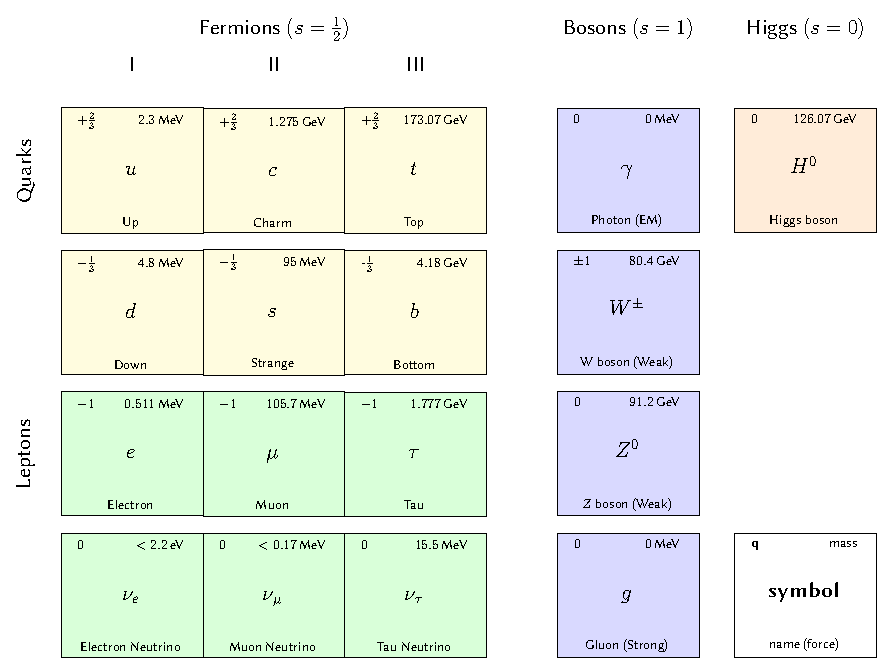
\includegraphics[width=\textwidth]{PartTheory/Diagrams/ParticleTable.pdf}
    \caption{A summary of all elementary particles described by the SM\cite{Theory:PDGBooklet}. Note the various groupings and divisions including by spin, generation and particle type. Within the fermion sector the quarks are shown in yellow and the leptons are shown in green. These are grouped into three different generations traditionally denoted by roman numerals. The force mediators known as gauge bosons are shown in blue and finally the recently discovered Higgs boson with a spin of zero.} \label{tab:TheorySmParticles}
\end{table}

%% Table of Forces
\begin{table}[htbp]
  \centering  
    \begin{tabular}{|c|c|c|}
    \hline
    Name & Relative Strength & Boson \\ \hline \hline
    Strong & $10^{38}$ & Gluons \\
    Electromagnetic & $10^{36}$ & Photon \\ 
    Weak & $10^{25}$ & \Wboson and \Zboson \\
    Gravity & $1$ & Graviton* \\ \hline
    \end{tabular}
    \caption{A summary of the four fundamental forces ordered by relative strength. These are approximate relative strengths for the purpose of demonstrating the hierarchy of forces as a function of their strength. A more accurate determination of the interaction strength depends on the details of the interaction itself. Note however the order-of-magnitude differences in the relative strengths of these forces. Note that the graviton is the theoretical boson responsible for mediating gravitational interactions, it is not part of the SM.} \label{tab:TheoryForces} 
\end{table}

\section{Quantum Electrodynamics}

The interaction of particles via the electromagnetic force is described by Quantum Electrodynamics or QED. These interactions are mediated by the massless neutral boson known as the photon and the strenght of the interaction is characterized by the fine-structure constant $\alpha$. All electrically charged fermions are allowed to interact, since the photon itself is not charged, no self-interaction is allowed within QED. Figure~\ref{fig:TheorySimpleQED} shows the single vertex described by QED, where two fermions interact via a photon. Note that the electric charge is conserved across the vertex, so for example $\gamma\rightarrow e^{+}e^{+}$ is not allowed within QED.

%% Simple QED Vertex
\begin{figure}
  \centering
  \begin{fmffile}{simpleqed}
  \fmfframe(7,6)(5,4) {
    \begin{fmfgraph*}(100,80)
      \fmftop{fi,fo} \fmfbottom{Photon}
      \fmf{fermion}{fi,vx1,fo}
      \fmf{boson,label=$\gamma$}{vx1,Photon}
      \fmflabel{$f$}{fi} \fmflabel{$f$}{fo}
      \fmfdot{vx1}
    \end{fmfgraph*}
    }
\end{fmffile}
  \caption{The interaction vertex described by QED. One can obtain all possible vertex shapes by rotating this basic vertex and assigning the appropriate electric charge and making sure to conserve lepton number across the vertex.} \label{fig:TheorySimpleQED}
\end{figure}

By combining different forms of this vertex one can build every possible QED interaction. For example an $e^{+}e^{-}$ pair can annihilate to create energy in the form of a photon as shown in Fig.~\ref{fig:TheoryQEDTreeA} and then subsequently decay into an additional $e^{+}e^{-}$ pair. Electrons can scatter by emitting a photon which is then absorbed by a positron as shown in Fig.~\ref{fig:TheoryQEDTreeB} this process is known as Bhabha scattering.

%% Example Tree Level Diagrams
\begin{figure}
  \centering
  \begin{minipage}[][][t]{.47\textwidth}
    \centering
    \begin{fmffile}{TheoryQEDTreeA}
\fmfframe(5,17)(20,17) {
\begin{fmfgraph*}(100,80)
\fmfleft{ele1,pos1}
\fmfright{ele2,pos2}
\fmf{fermion}{ele1,v1}
\fmf{fermion}{v1,pos1}
\fmf{photon,label=$\gamma$}{v1,v2}
\fmf{fermion}{ele2,v2}
\fmf{fermion}{v2,pos2}
\fmflabel{$e^{+}$}{pos1} \fmflabel{$e^{+}$}{pos2}
\fmflabel{$e^{-}$}{ele1} \fmflabel{$e^{-}$}{ele2}
\fmfdot{v1,v2}
\end{fmfgraph*}
}
\end{fmffile}
    \subcaption{Electron-Positron pair annihilation mediated by a photon.} \label{fig:TheoryQEDTreeA}
  \end{minipage}
  \,
  \begin{minipage}[][][t]{.47\textwidth}
    \centering
    \begin{fmffile}{TheoryQEDTreeB}
\fmfframe(5,17)(20,17) {
\begin{fmfgraph*}(100,80)
\fmfleft{ele1,pos1}
\fmfright{ele2,pos2}
\fmf{fermion}{ele1,v1}
\fmf{fermion}{v1,ele2}
\fmf{photon,label=$\gamma$}{v1,v2}
\fmf{fermion}{v2,pos1}
\fmf{fermion}{pos2,v2}
\fmflabel{$e^{+}$}{pos1} \fmflabel{$e^{+}$}{pos2}
\fmflabel{$e^{-}$}{ele1} \fmflabel{$e^{-}$}{ele2}
\end{fmfgraph*}
}
\end{fmffile}
    \subcaption{Electron-Positron pair scattering via the emission of a photon.} \label{fig:TheoryQEDTreeB}
  \end{minipage}
  \caption{Feynman diagrams of the process $e^{+}e^{-}\rightarrow e^{+}e^{-}$ allowed in QED. Note that these are the simplest diagrams, also known as tree level diagrams, and additional vertices can be added to produce higher-order diagrams of the same process.}
  \label{fig:TheoryQEDTree}
\end{figure}

\section{Quantum Chromodynamics}

Interactions via the strong force are described in the theory of Quantum Chromodynamics or QCD. These interactions are mediated by a set of massless neutral bosons known as gluons. QCD introduces the concept of colour, which similarly to electrical charge, determines the possible interactions that can occur via the strong force. Colour can take three states: red (antired), blue (antiblue), green (antigreen):

For example both quarks and gluons possess colour and as a result gluons, unlike photons, can self-interact in a three gluon vertex (Figure~\ref{fig:TheoryQCDThreeGluon}) or a four gluon vertex (Figure~\ref{fig:TheoryQCDFourGluon}). As with electrical charge, colour-charge must also be conserved. Thus in the scattering process $q\rightarrow q+g$ shown in Figure~\ref{fig:TheoryQCDColour} the flavour of the quark may not change but the colour-charge does and the gluon carries away the difference in colour. Thus each gluon has two color charges associated it. Naively one would expect nine different types of gluon that participate in interaction, owing to the nine possible combinations of colour and anticolour, however the SU(3) symmetry on which QCD is based results in a colour octet:
\begin{equation*}
\begin{aligned}[c]
  &(r\overline{b}+b\overline{r})/\sqrt{2} \\
  -i&(r\overline{b}-b\overline{r})/\sqrt{2} \\
  &(r\overline{r}+b\overline{b})/\sqrt{2} \\
  &(r\overline{g}+g\overline{r})/\sqrt{2}
\end{aligned}
\qquad\qquad
\begin{aligned}[c]
  -i&(r\overline{g}-g\overline{r})/\sqrt{2} \\
  &(b\overline{g}+g\overline{b})/\sqrt{2} \\
  -i&(b\overline{g}-g\overline{b})/\sqrt{2} \\
  &(r\overline{r}+b\overline{b}-2g\overline{g})/\sqrt{6}
\end{aligned}
\end{equation*}
%
and a ``colour singlet'':
%
\begin{equation}
  (r\overline{r} + g\overline{g} + b\overline{b})/\sqrt{3}
\end{equation}
%
which is overall colourless.

There are then eight different gluons that can participate in QCD interactions each with a different colour-charge combination. Additionally there is a ninth combination which is overall colorless so it cannot take part in interactions.

In an analogous fashion to screening which occurs with electric charges, quark-antiquark pairs act like dipoles which screen the true colour charge of the central quark. However since gluons also carry colour, they cause the opposite effect (anti-screening) to amplify and change the observed colour of the quark. Which effect wins out depends on the number of colours in the theory and the number of quark flavours. As it is with three colour states and six different quark flavours, anti-screening is the overall dominant effect. As a result the colour potential decreases with distance and quarks experience very little potential when very near to each other. This effect is known as asymptotic freedom and results in quarks only existing within colorless bound states known as \textit{hadrons}.

Hadrons can be divided into two categories: \textit{mesons}, which contain a quark and an antiquark ($q\overline{q}$); and \textit{baryons} which are made of three quarks (or antiquarks) each with a different (anti)colour-charge to result in a colourless composite particle. Common examples of baryons are protons ($uud$) and neutrons ($udd$) which are the building blocks of atomic nuclei. While $\pi^{0}$ ($u\overline{u}/d\overline{d}$) is a commonly produced meson in hadron colliders. Note that due to the quark configuration, baryons have baryon number $B=+1$ while mesons have $B=0$.
  
%% Self-interacting QCD Gluon vertices
\begin{figure}
  \begin{minipage}[][][t]{.32\textwidth}
    \begin{fmffile}{ColourQCD}
\begin{fmfgraph*}(100,80)
\fmftop{qin,qout} \fmfbottom{glu}
\fmf{quark}{qin,vertex1,qout}
\fmf{gluon,label=$g$,l.d=10}{vertex1,glu}
\fmfdot{vertex1}
\fmflabel{$q$}{qin} \fmflabel{$q$}{qout}
\end{fmfgraph*}
\end{fmffile}
    \subcaption{Quark-gluon vertex.} \label{fig:TheoryQCDColour}
  \end{minipage}
  \,
  \begin{minipage}[][][t]{.32\textwidth}
    \centering
    \begin{fmffile}{selfqcd4}
\fmfframe(5,17)(20,17) {
\begin{fmfgraph*}(100,80)
\fmfleft{glu1,glu2}
\fmfright{glu3,glu4}
\fmf{gluon}{vertex1,glu1} \fmf{gluon}{vertex1,glu2}
\fmf{gluon}{glu3,vertex1} \fmf{gluon}{glu4,vertex1}
\fmfdot{vertex1}
\fmflabel{$g$}{glu1} \fmflabel{$g$}{glu2}
\fmflabel{$g$}{glu3} \fmflabel{$g$}{glu4}
\end{fmfgraph*} 
}
\end{fmffile}
    \subcaption{Four-gluon vertex} \label{fig:TheoryQCDFourGluon}
  \end{minipage}
  \,
  \begin{minipage}[][][t]{.32\textwidth}
    \centering
    \begin{fmffile}{selfqcd3}%
  \fmfframe(6,10)(1,10) {%
    \begin{fmfgraph*}(100,80)%
      \fmfleft{glu1}
      \fmfright{glu3,glu4}
      \fmf{gluon}{vertex1,glu1}
      \fmf{gluon}{glu3,vertex1} \fmf{gluon}{glu4,vertex1}
      \fmfdot{vertex1}
      \fmflabel{$g$}{glu1}
      \fmflabel{$g$}{glu3}
      \fmflabel{$g$}{glu4}
    \end{fmfgraph*}%
  }%
\end{fmffile}%
    \subcaption{Three-gluon vertex} \label{fig:TheoryQCDThreeGluon}
  \end{minipage}
  \caption{Diagrams of the fundamental interaction vertices described by quantum chromodynamics.} \label{fig:TheoryQCDVertexes}
\end{figure}

\section{Weak Interactions} \label{sec:TheoryWeakInteractions}

The final type of interaction involves the so-called weak force. The weak force is responsible for $\beta^{-}$ decay ($n\rightarrow p +e^{-}+\overline{\nu}_{e}$) and $\beta^{+}$ decay. Interactions via the weak force are mediated by a single neutral massive boson and two charged massive bosons. Since the bosons responsible for weak interactions are massive, the range of interaction is very short, unlike electromagnetic interactions via a massless photon.

All fermions can take part in interactions via the weak force. Let us consider weak interactions involving only leptons. The weak neutral vertex is very similar to the basic vertex seen in QED (\ref{fig:TheorySimpleQED}) A valid interactions via the weak force is then formed by combining these simple vertices (Figure~\ref{fig:TheoryWeakVertexes}) while taking care to conserve electric charge and lepton flavour. An example of a leptonic weak interaction is muon decay ($\mu\rightarrow \nu_{\mu}W^{-}\rightarrow \nu_{\mu}e^{-}\overline{\nu}_{e}$) shown in Figure~\ref{fig:TheoryMuonDecay}.

%% Weak Neutral Vertexes
\begin{figure}
  \begin{minipage}[][][t]{.32\textwidth}
    \centering
    \begin{fmffile}{WeakNeutral}
  \fmfframe(5,10)(6,10) { % left, top, right, bottom
    \begin{fmfgraph*}(100,80)
      \fmftop{fi,fo} \fmfbottom{ZBoson}
      \fmf{fermion}{fi,vx1,fo}
      \fmf{boson,label=$Z^{0}$}{vx1,ZBoson}
      \fmflabel{$f$}{fi} \fmflabel{$\overline{f}$}{fo}
      \fmfdot{vx1}
    \end{fmfgraph*}
  }
\end{fmffile}
    \subcaption{Neutral current weak vertex} \label{fig:TheoryWeakNeutralFermions}
  \end{minipage}
  \,
  \begin{minipage}[][][t]{.32\textwidth}
    \centering
    \begin{fmffile}{WeakCharged}
\begin{fmfgraph*}(100,80)
\fmftop{fi,fo} \fmfbottom{WBoson}
\fmf{fermion}{fi,vx1,fo}
\fmf{boson,label=$W$}{vx1,WBoson}
\fmflabel{$\ell$}{fi} \fmflabel{$\nu_{\ell}$}{fo}
\fmfdot{vx1}
\end{fmfgraph*}
\end{fmffile}
    \subcaption{Charged current vertex involving leptons} \label{fig:TheoryWeakChargedLeptons}
  \end{minipage}
  \,
  \begin{minipage}[][][t]{.32\textwidth}
    \centering
    \begin{fmffile}{WeakChargedQuark}
  \fmfframe(5,10)(6,10) {%
    \begin{fmfgraph*}(100,80)
      \fmftop{fi,fo} \fmfbottom{WBoson}
      \fmf{fermion}{fi,vx1,fo}
      \fmf{boson,label=$W$}{vx1,WBoson}
      \fmflabel{$\overline{q}$}{fi} \fmflabel{$q'$}{fo}
      \fmfdot{vx1}
    \end{fmfgraph*}
  }
\end{fmffile}
    \subcaption{Charged current vertex involving quarks} \label{fig:TheoryWeakChargedQuarks}
  \end{minipage}

  \caption{The neutral current and charged current vertices allowed via the weak force. Where $f$ can be an $e$, $\mu$ or $\tau$ and $\nu_{\ell}$ is the corresponding lepton neutrino of the same flavour. 
  One can obtain all possible interaction vertices by rotating these basic vertices and assigning the appropriate electric charge and making sure to conserve lepton flavour across the vertex.} \label{fig:TheoryWeakVertexes}
\end{figure}

%% Weak Muon Decay
\begin{figure}
  \centering
  \begin{fmffile}{WeakMuonDecay}
\begin{fmfgraph*}(150,75)
\fmfbottom{mu,d1,munu}
\fmfright{d0,e,enu}
\fmf{fermion}{mu,v1,munu} 
\fmffreeze
\fmf{fermion}{e,v2,enu}
\fmf{boson,tension=1.5,label=$W^-$}{v1,v2}
\fmflabel{$e^{-}$}{e}
\fmflabel{$\overline{\nu}_{e}$}{enu}
\fmflabel{$\mu^-$}{mu}
\fmflabel{$\nu_{\mu}$}{munu}
\fmfdot{v1,v2}
\end{fmfgraph*}
\end{fmffile}
  \caption{Neutral current weak scattering vertex} \label{fig:TheoryMuonDecay}
\end{figure}

Let us consider weak interactions involving quarks. The neutral vertex is similar to that of the leptonic version, a quark can emit a \ZbosonText{} or a \ZbosonText{} can decay forming a quark-antiquark pair. The charged current then changes the flavour of an up-type quark into a down-type quark (or vice-versa) with a \WbosonText{} of the appropriate charge (Figure~\ref{fig:TheoryWeakChargedQuarks}). It is possible for a weak interaction to change the flavour of a quark across families. A well known example of such an interaction is Kaon decay ($K^{+}\rightarrow \mu^{+}\nu_{\mu}$). In order to account for this interaction and preserve the universality of weak interactions, Nicola Cabibbo postulated\cite{Theory:CKMNicola} that the states that the states that couple to the charged current are really a mixture of 'rotated' quark states:

\begin{equation}
\begin{pmatrix}
  u \\
  d' \\
\end{pmatrix}
\begin{pmatrix}
  c \\
  s' \\
\end{pmatrix}
\end{equation}

where

\begin{subequations}
  \begin{equation}
  \label{eq:TheoryWeakQuarkMixingEq1}
  d'=d\cos\theta_{c} + s\sin\theta_{c}
  \end{equation}
  \begin{equation}
  \label{eq:TheoryWeakQuarkMixingEq2}
  s'=-d\sin\theta_{c} + s\cos\theta_{c}
  \end{equation}
\end{subequations}

This introduces an arbitrary parameter into the theory known as the quark mixing angle or the Cabibbo angle, named after Nicola Cabibbo who developed the phenomenon of quark mixing. The introduction of quark mixing has the effect of attenuating the interaction strength at vertices involving multiple quark generations. Interactions which cross one generation are said to be Cabibbo Suppressed while those that cross two generations are Doubly Cabibbo suppressed.

Taking into account the three quark generations, quark mixing can be expressed in matrix notation as shown in Equation~\ref{eq:TheoryWeakQuarkMixingMatrix}. This unitary matrix is known as the Cabibbo-Kobayashi-Maskawa Matrix (CKM Matrix) after Cabibbo which initially postulated quark mixing and Makoto Kobayashi and Toshihide Maskawa who later added an additional generation, containing the top and bottom quarks, to the matrix\cite{Theory:CKMKobayashiMaskawa}.

\begin{equation}
\label{eq:TheoryWeakQuarkMixingMatrix}
\begin{pmatrix}
  d' \\
  s' \\
  b' \\
\end{pmatrix}
=
V_{CKM}
\begin{pmatrix}
  d \\
  s \\
  b \\
\end{pmatrix}
=
\begin{pmatrix}
  V_{ud} & V_{us} & V_{ub} \\
  V_{cd} & V_{cs} & V_{cb} \\
  V_{td} & V_{ts} & V_{tb} \\
\end{pmatrix}
\begin{pmatrix}
  d \\
  s \\
  b \\
\end{pmatrix}
\end{equation}

Several parameterizations of the CKM matrix exist, the ``standard'' parametrization uses angles $\theta_{\textrm{12}}$, $\theta_{\textrm{23}}$, $\theta_{\textrm{13}}$ and a phase $\delta_{\textrm{13}}$:

\begin{equation}
\label{eq:TheoryWeakCKMStandard}
V_{CKM}
=
\begin{pmatrix}
c_{12}c_{13} & s_{12}c_{13} & s_{13}\exp(-i\delta) \\
-s_{12}c_{23}-c_{12}s_{23}s_{13}\exp(i\delta) & c_{12}c_{23} - s_{12}s_{23}s_{13}\exp(i\delta) & s_{23}c_{13} \\ 
s_{12}s_{23}- c_{12}c_{23}s_{13}\exp(i\delta) & -c_{12}s_{23}-s_{12}c_{23}s_{13}\exp(i\delta) & c_{23}c_{13} \\
\end{pmatrix}
\end{equation}

where $c_{ij}=\cos\theta_{ij}$ and $s_{ij}=\sin\theta_{ij}$ for i=1,2,3. This parametrization has the advantage that each angle $\theta_{ij}$ relates to a specific transition from one generation to the other. If $\theta_{13} = \theta_{23} = 0$ the third generation is not coupled to the other two and the matrix reduces to the original matrix postulated by Cabibbo. Note that $\theta_{12}$ is the Cabibbo angle, $\theta_c$, described earlier.

Another parameterization due to Wolfenstein \cite{Theory:CKMWolfenstein} expresses all elements in terms of the Cabibbo angle by defining $\lambda\equiv s_{12}=\sin \theta_{12}$ and then expressing the other elements in terms of powers of $\lambda$:

\begin{equation}
\label{eq:TheoryWeakCKMWolfenstein}
V_{CKM}
\approx
\begin{pmatrix}
1-\lambda^2/2 & \lambda & A\lambda^3(\rho-i\eta) \\
-\lambda & 1-\lambda^2/2 & A\lambda^2 \\ 
A\lambda^3(1-\rho-i\eta) & -A\lambda^2 & 1\\
\end{pmatrix}
\end{equation}
%
where A, $\rho$ and $\eta$ are all real numbers intended to express the order of magnitude differences between $s_{12}$ and the other elements in the matrix. Of course, all the elements should be the same irrespective of which parametrization is used.

The elements of the CKM matrix have been measured and the latest accepted results are summarized in \ref{eq:TheoryWeakCKM}\cite{Theory:PDGBooklet}. The interaction strength is then proportional to $|V_{ij}|^{2}$. Including all three generations the sum of all possible transitions from a given quark, q, is unity:

\begin{equation} 
  \label{eq:TheoryWeakMixingTotal}
  \sum|V_{qi}|^{2}=1
\end{equation}

Note that the term $V_{tb}$ is approximately unity and by far dominates over the other $V_{tj}$ terms. This means that the top-quark transitions almost exclusively into a $b$-quark ($t\rightarrow Wb$) with transitions $t\rightarrow Ws$ and $t\rightarrow Wd$ being exceedingly rare. The soft muon tagger which is the focus of this thesis relies on weak semileptonic decays of $b$-quarks. From~\ref{eq:TheoryWeakCKM} one can see that the transition $b\rightarrow c$ dominates over $b\rightarrow u$. Additionally the focus of this theses is on semileptonic \ttbar\ events, where one of the $W$ bosons in the event decays to quarks as per the magnitude of $V_{ij}$.

\begin{equation}
\label{eq:TheoryWeakCKM}
V_{CKM}
=
\begin{pmatrix}
  0.97427\pm0.00015 & 0.22534\pm0.00065 & 0.00351\substack{+0.00015\\-0.00014} \\
  0.22520\pm0.00065 & 0.97344\pm0.00016 & 0.0412\substack{+0.0011\\-0.0005} \\
  0.00867\substack{+0.00029\\-0.00031} & 0.0404\substack{+0.0011\\-0.0005} & 0.999146\substack{+0.000021\\-0.000046} \\
\end{pmatrix}
\end{equation}

An additional unique feature of weak interactions is that the charge conjugation-parity ($CP$) symmetry is violated. The operator $C$ denotes the change of a particle by its antiparticle partner and $P$ denotes a reversal of helicity (the projection of spin onto the momentum of a particle). A clear violation of $C$ and $P$ was observed in the radioactive decay of Cobalt-60, where the resulting electrons were preferentially emitted in the opposite direction of the nuclear spin of the Cobalt. Thus weak currents only couple to left-handed neutrinos (or right-handed antineutrinos) this is then a violation of parity. Additionally charge symmetry is also violated since a left-handed neutrino is preferentially picked over a left-handed antineutrino. Finally in 1964 $CP$ violation was observed in the decay of neutral kaon.

Thus the probability of $\overline{a}\rightarrow \overline{b}$ is not equal to that of $a\rightarrow b$. The existence of $CP$ violation has interesting consequences for the formation of the early universe. The preferential production of matter over antimattter in $CP$ violating interactions would shift the balance in favour of matter resulting in a universe similar to our own. Finally as with QCD, weak interactions couple weak bosons to each other. Thus the vertex $Z\rightarrow W^-W^+$ is allowed via the weak force.

\subsection{Electroweak Unification and the Higgs mechanism}

The unification of the electromagnetic and weak theories was first proposed by Glashow and later developed by Weinberg and Salam into the electroweak theory. The theory postulates that while at low energies the two forces are to be treated separately, at higher the two can be seen as a single force. Thus the two forces are different manifestation of the same ``electroweak'' interaction. There were several stumbling blocks to the unification of the forces. Firstly, the boson which drives the electromagnetic interaction, the photon, is massless while the weak bosons are both massive. Evidence for the massive nature of these bosons has been established by experimental results from \comment{Cite W and Z experiments} at CERN.

Thus the symmetry of the theory must be spontenously broken in some way. A mechanism for ElectroWeak Symmetry Breaking (EWSB) was postulated by Higgs, Brout, Englert and others which introduces massess to the weak bosons and posits the existence of an additional scalar (spin $S=0$) boson known as the Higgs boson.

\subsubsection{Gauge Theories}

Gauge invariance is one of the underlying invariances which underpins the Standard Model. Given the so-called Dirac lagrangian\footnote{A Lagrangian is a mathematical function that describes the underlying dynamics of a system as a function of time and space coordinates ($x^{\mu}$) and their time derivatives.}

\begin{equation}
  \label{eq:TheoryHiggsDiracLagrangian}
  \Lagr = i\hbar c \overline{\psi}\gamma^{\mu}\partial_{\mu}\psi -mc^2\overline{\psi}\psi
\end{equation}
%
which describes a free particle of spin-$\frac{1}{2}$ with mass $m$. Note that it is invariant under the transformation
%
\begin{equation}
  \psi\rightarrow e^{i\theta}\psi\textrm{, where $\theta$ is a real number}
\end{equation}
%
since the adjoint $\overline{\psi}\rightarrow e^{-i\theta}\overline{\psi}$ and the two terms cancel out. This is known as a \emph{(global) gauge transformation}. This is essentially a phase transformation which is constant everywhere. Meaning the phase change is the same in all points of space-time. A ``local'' gauge transformation occurs when the phase is different for different points in space-time:
%
\begin{equation}
  \psi\rightarrow e^{i\theta(x)}\psi
\end{equation}

Note that the Dirac lagrangian (Equation~\ref{eq:TheoryHiggsDiracLagrangian}) is then not invariant under a local gauge transformation since extra terms are created by the derivative. This then implies that the underlying physics of such a theory depends ones position in space-time. Thus local gauge invariance must be imposed. In the case of the Dirac lagrangian, this is done by introducing additional terms to the Dirac lagrangian which will cancel the extra terms introduced by the local gauge transformation. As it turns out this results in the introduction of a new massless vector field that couples to $\psi$.

The new lagrangian then describes a spin-$\frac{1}{2}$ particle with mass $m$ that interacts with a free massless field. This new field can be indentified as the electromagnetic field and the spin-$\frac{1}{2}$ particles are electrons and positrons. Thus the resulting lagrangian describes all interactions that form part of quantum electrodynamics.

A similar procedure can be applied to the color quark model and obtain a description of all QCD interactions. However requiring that the weak theory be a gauge theory (invariant under local gauge transformation) encounters a problem since the weak bosons are known to be massive. There must be some mechanism via which the $W^{\pm}$ and $Z^0$ obtain mass.

The Higgs mechanism posits the existence of a complex scalar field doublet that when introduced into the electroweak Lagrangian results in the weak fields acquiring a mass term. In other words the $W^{\pm}$ and $Z^{0}$ interact with the Higgs field and obtain a mass. An additional consequence of introducing the Higgs field is the inclusion of a scalar boson particle, the the so-called ``Higgs boson''. Finally the Higgs field also couples to fermions via the Yukawa coupling generating gauge invariant mass terms for the fermions as well.\footnote{For a more complete description of the mathematical procedure see~\cite{Theory:IntroGriffiths}.}.

The SM Lagrangian in its current form including the Higgs potential is shown in Equation~\ref{eq:TheorySMLagrangian}. This expression describes all possible particle interactions that form part of the SM, of particular interest are the fermion mass term which couples the fermion field ($\psi$) to the scalar Higgs field ($\phi$) and the Higgs kinetic and potential terms.

\begin{align}
  \Lagr = &- \underbrace{ \frac{1}{4} W^a_{\mu\nu} W^{\mu\nu a} }_{ \text{Weak Field} }
           - \underbrace{ \frac{1}{4} B_{\mu\nu} B^{\mu\nu} }_{ \text{EM Field} }
           - \underbrace{ \frac{1}{4} G^a_{\mu\nu} G^{\mu\nu a} }_{ \text{Strong Field} } \nonumber \\
          &+ \underbrace{ \overline{\psi}\slashed{D}_{\mu}\psi}_{ \text{Fermion Kinetic} }
           + \underbrace{ \lambda\overline{\psi}\psi\phi }_{ \text{Fermion Mass} } \label{eq:TheorySMLagrangian} \\
          &+ \underbrace{ |D_{\mu}\phi^2| }_{ \text{Higgs Kinetic} }
           - \underbrace{ V(\phi) }_{ \text{Higgs Potential} } \nonumber
\end{align}
